\section{第6章\quad 实用微波传输线与波导}
\begin{frame}{第6章\quad 实用微波传输线与波导}
    \begin{itemize}
        \item 微波工程分析方法
              \begin{itemize}
                  \item 场论的方法
                  \item 网络的方法
              \end{itemize}
    \end{itemize}
    \begin{itemize}
        \item 传输线理论 $\Longrightarrow$ 波导
              \begin{itemize}
                  \item 当其他人或物靠近双导线时会产生较大影响。这说明,传输线与外界有能量交换,它带来的直接问题是能量损失和工作不稳定。就其原因是\textbf{开放(Open)}造成的特点
              \end{itemize}
    \end{itemize}
\end{frame}

\begin{frame}{第6章\quad 实用微波传输线与波导}
    \begin{itemize}
        \item 波导(Waveguide)构成
    \end{itemize}
    双导线两侧连续加对称$\lambda/4$支节,直到构成封闭(Closed)电路为止。如果其导线的宽度是$W$,则波导宽边
    \begin{align*}
        a=W+2\cdot \frac{\lambda}{4}=W+\frac{\lambda}{2} \\
        a\geqslant \lambda/2 或 \lambda\leqslant 2a
    \end{align*}
    这构成了波导传输的第一个约束条件 \\
    \centering
    \begin{figure}
        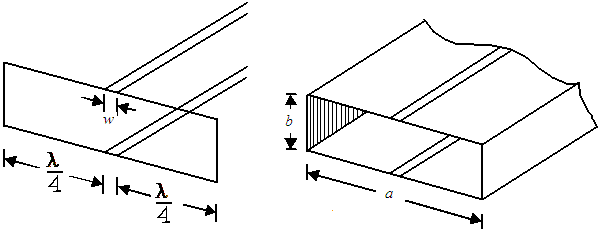
\includegraphics[width=6cm]{Cha6//fig6-0.png}
        \caption{从双导线到矩形波导}
    \end{figure}
\end{frame}

\subsection{预备知识}
\begin{frame}{预备知识}
    \begin{itemize}
        \item 交变电磁场基本关系式
    \end{itemize}
    \begin{align*}
        \begin{cases}
            \nabla\times\vec{E}=-\dfrac{\partial \vec{B}}{\partial t}        \\
            \nabla\times\vec{H}=\dfrac{\partial \vec{D}}{\partial t}+\vec{J} \\
            \nabla\cdot\vec{D}=\rho                                          \\
            \nabla\cdot\vec{B}=0
        \end{cases}
    \end{align*}
    \begin{align*}
        \vec{D}=\epsilon\vec{E},\vec{B}=\mu\vec{H},\vec{J}=\sigma\vec{E}
    \end{align*}
    无源区,时谐场
    \begin{align*}
        \begin{cases}
            \nabla\times\vec{E}=-\rm{j}\omega\mu\vec{H}     \\
            \nabla\times\vec{H}=\rm{j}\omega\epsilon\vec{E} \\
            \nabla\cdot\vec{D}=0                            \\
            \nabla\cdot\vec{B}=0
        \end{cases}
    \end{align*}
\end{frame}

\begin{frame}{预备知识}
    \begin{itemize}
        \item 边界条件
    \end{itemize}
    \begin{columns}
        \begin{column}{0.5\linewidth}
            两种媒质界面的边界条件
            \begin{align*}
                \begin{cases}
                    \hat{n}\times(\vec{E_2}-\vec{E_1})=0         \\
                    \hat{n}\times(\vec{H_2}-\vec{H_1})=\vec{J_s} \\
                    \hat{n}\cdot(\vec{D_2}-\vec{D_1})=\rho_s     \\
                    \hat{n}\cdot(\vec{B_2}-\vec{B_1})=0
                \end{cases}
            \end{align*}
        \end{column}
        \begin{column}{0.5\linewidth}
            理想导体表面的边界条件
            \begin{align*}
                \begin{cases}
                    \hat{n}\times\vec{E_2}=0         \\
                    \hat{n}\times\vec{H_2}=\vec{J_s} \\
                    \hat{n}\cdot\vec{D_2}=\rho_s     \\
                    \hat{n}\cdot\vec{B_2}=0
                \end{cases}
            \end{align*}
        \end{column}
    \end{columns}
\end{frame}

\begin{frame}
    \begin{itemize}
        \item 交变电磁场的能量关系
    \end{itemize}
    对于一封闭曲面S,电磁场的能量关系满足复功率定理,即
    \begin{align*}
        -\oint_S\frac{1}{2}(\vec{E}\times\vec{H^*})\cdot\hat{n}\rm{d}S=P_L+\rm{j}2\omega(W_m-W_e)
    \end{align*}
\end{frame}

\begin{frame}{预备知识}
    \begin{itemize}
        \item 导波系统波型\\
              导波系统中的电磁波按纵向场分量的有无,分为以下三种波型(模)
              \begin{itemize}
                  \item 横磁波(TM波),又称电波(E波): $H_z=0,E_z\neq 0$
                  \item 横电波(TE波),又称磁波(H波): $E_z=0,H_z\neq 0$
                  \item 横电磁波(TEM波): $E_z=0,H_z=0$
              \end{itemize}
    \end{itemize}
\end{frame}

\begin{frame}{预备知识}
    \begin{itemize}
        \item 波导一般解的出发点和假定条件\\
              波导一般解的出发点是频域Maxwell方程组
              \begin{align}
                  \begin{cases}
                      \nabla\times\vec{H}=\rm{j}\omega\epsilon\vec{E} \\
                      \nabla\times\vec{E}=-\rm{j}\omega\mu\vec{H}     \\
                      \nabla\cdot\vec{E}=0                            \\
                      \nabla\cdot\vec{H}=0
                  \end{cases}
                  \label{eqn6-1}
              \end{align}
              波导假定条件
              \begin{columns}
                  \begin{column}{0.5\linewidth}
                      \begin{itemize}
                          \item 波导均匀条件:假定横截面不随$z$而变化
                          \item 媒质均匀条件:波导内部$\epsilon,\mu$均匀,波导内壁$\sigma$无限大
                          \item 无源条件:波导内$\rho,\vec{J}\equiv 0$
                          \item 无限条件:波导在$z$方向无限长
                      \end{itemize}
                  \end{column}
                  \begin{column}{0.5\linewidth}
                      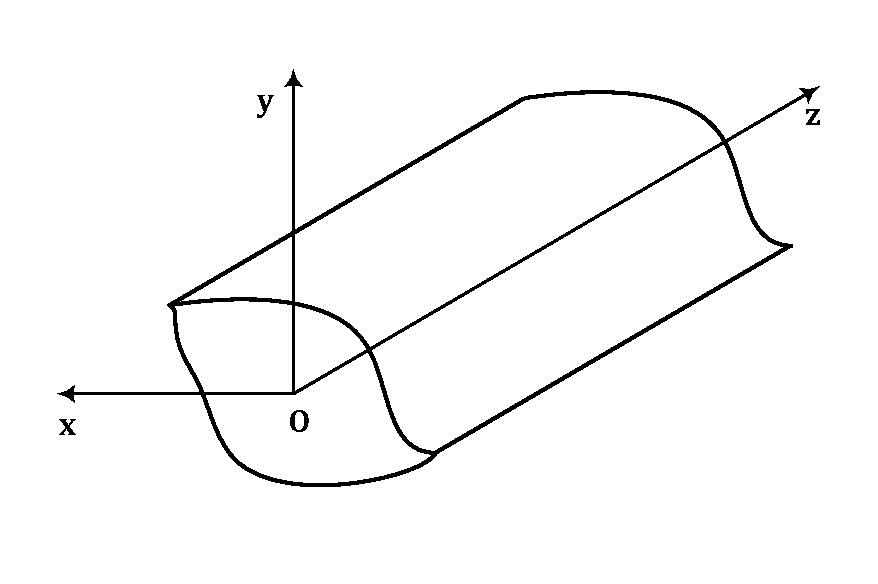
\includegraphics[width=5cm]{Cha6//fig6-1.pdf}
                  \end{column}
              \end{columns}
    \end{itemize}
\end{frame}

\subsection{矩形波导}

\begin{frame}{矩形波导}
    \begin{itemize}
        \item 矩形波导的一般解
    \end{itemize}
    (\ref{eqn6-1})第二式两边取旋度
    \begin{align*}
        \nabla\times\nabla\times\vec{E} & =\nabla(\nabla\cdot\vec{E})-\nabla^2\vec{E}=-\rm{j}\omega\mu\nabla\times\vec{H} \\
                                        & =\omega^2\mu\epsilon\vec{E}=k^2\vec{E}                                          \\
                                        & k=\omega\sqrt{\mu\epsilon}=2\pi/\lambda
    \end{align*}
    得到波动方程
    \begin{align}
        \begin{cases}
            \nabla^2\vec{E}+k^2\vec{E}=0 \\
            \nabla^2\vec{H}+k^2\vec{H}=0 \\
        \end{cases}\label{eqn6-2}
    \end{align}
\end{frame}

\begin{frame}{矩形波导}
    \begin{itemize}
        \item 纵向场表示横向场
    \end{itemize}
    \centering
    \begin{figure}
        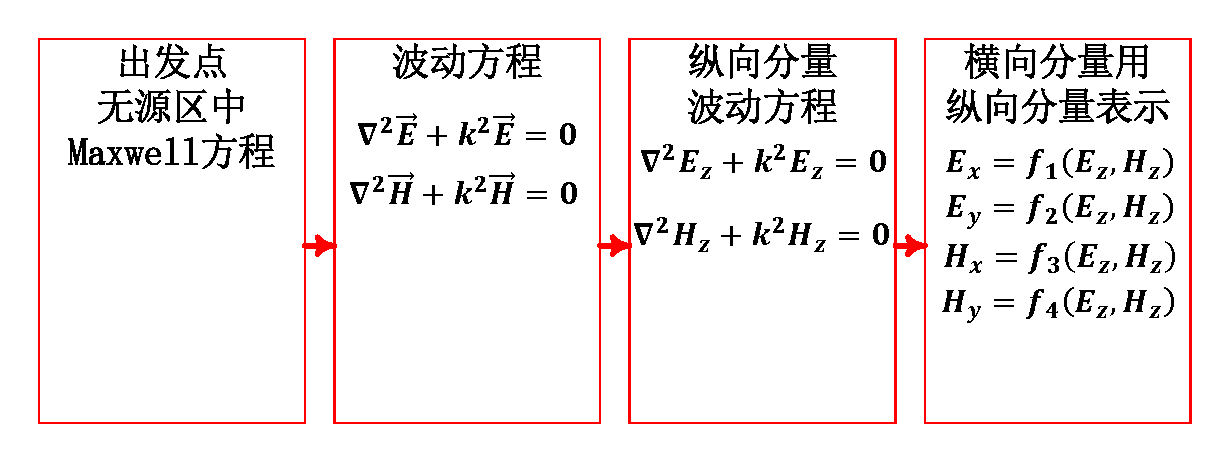
\includegraphics[width=10cm]{Cha6/fig6-2.pdf}
        \caption{纵向分量法流程图}   %\numberwithin{figure}{section}
    \end{figure}
\end{frame}

\begin{frame}{矩形波导}
    纵向分量方程
    \begin{align}
        \begin{cases}
            \nabla^2E_z+k^2E_z=0 \\
            \nabla^2H_z+k^2H_z=0
        \end{cases}
        \label{eqn6-3}
    \end{align}
    假定$E_z$或$H_z$可分离变量,即
    \begin{align}
        \begin{cases}
            E_z=E(x,y)Z(z) \\
            H_z=H(x,y)W(z)
        \end{cases}
        \label{eqn6-4}
    \end{align}
    且$Laplace$算子$\nabla^2$可分解为
    \begin{align}
        \nabla^2=\nabla_t^2+\frac{\partial^2}{\partial z^2}
        \label{eqn6-5}
    \end{align}
    将式(\ref{eqn6-4})、式(\ref{eqn6-5})代入式(\ref{eqn6-3})可知
\end{frame}

\begin{frame}{矩形波导}
    \begin{align}
        \frac{\nabla^2_t E(x,y)}{E(x,y)}+\frac{1}{Z(z)}\frac{\rm{d}^2 Z(z)}{\rm{d}z^2}+k^2=0
        \label{eqn6-6}
    \end{align}
    由于其独立性,上式各项均为常数
    \begin{align}
        \begin{cases}
            \dfrac{1}{Z(z)}\dfrac{\rm{d}Z(z)}{\rm{d}z^2}=\gamma^2 \\
            \dfrac{\nabla_t^2E(x,y)}{E(x,y)}+k_c^2=0
        \end{cases}
        \label{eqn6-7}
    \end{align}
    其中
    \begin{align}
        k_c^2=k^2+\gamma^2
    \end{align}
    称为\textbf{截止波数}
\end{frame}

\begin{frame}{矩形波导}
    式(\ref{eqn6-7})中第一方程的解是
    \begin{align}
        Z(z)=C_1\rm{e}^{-\gamma z}+C_2\rm{e}^{\gamma z}
    \end{align}
    有趣的是:波导解的$z$函数与传输线解有惊人的相似,又是入射波和反射波的组合。我们只研究一个波(不论是TE或TM波),在形式上只写入射波
    \begin{align}
        \begin{cases}
            E_z=E(x,y)\rm{e}^{-\gamma z} \\
            H_z=H(x,y)\rm{e}^{-\gamma z}
        \end{cases}
    \end{align}
    $$\frac{\partial}{\partial z}\rightarrow -\gamma$$ 
\end{frame}

\begin{frame}{矩形波导}
    \begin{align*}
        \nabla\times\vec{H}=\rm{j}\omega\epsilon \vec{E}
    \end{align*}
    \begin{align*}
         & \begin{vmatrix}
               \hat{x}                      & \hat{y}                      & \hat{z} \\
               \dfrac{\partial}{\partial x} & \dfrac{\partial}{\partial y} & -\gamma \\
               H_x                          & H_y                          & H_z     \\
           \end{vmatrix}
        =\rm{j}\omega\epsilon(\hat{x}E_x+\hat{y}E_y+\hat{z}E_z)
    \end{align*}
    \begin{align}
        \begin{cases}
            \dfrac{\partial H_z}{\partial y}+\gamma H_y=\rm{j}\omega\epsilon E_x  \\
            -\gamma H_x-\dfrac{\partial H_z}{\partial x}=\rm{j}\omega\epsilon E_y \\
            \dfrac{\partial H_y}{\partial x}-\dfrac{\partial H_x}{\partial y}=\rm{j}\omega\epsilon E_z
        \end{cases}
    \end{align}
\end{frame}

\begin{frame}{矩形波导}
    \begin{align*}
        \nabla\times\vec{E}=-\rm{j}\omega\mu \vec{H}
    \end{align*}
    \begin{align*}
        \begin{vmatrix}
            \hat{x}                      & \hat{y}                      & \hat{z} \\
            \dfrac{\partial}{\partial x} & \dfrac{\partial}{\partial y} & -\gamma \\
            E_x                          & E_y                          & E_z     \\
        \end{vmatrix}
        =-\rm{j}\omega\mu(\hat{x}H_x+\hat{y}H_y+\hat{z}H_z)
    \end{align*}
    \begin{align}
        \begin{cases}
            \dfrac{\partial E_z}{\partial y}+\gamma E_y=-\rm{j}\omega\mu H_x  \\
            -\gamma E_x-\dfrac{\partial E_z}{\partial x}=-\rm{j}\omega\mu H_y \\
            \dfrac{\partial E_y}{\partial x}-\dfrac{\partial E_x}{\partial y}=-\rm{j}\omega\mu H_z
        \end{cases}
    \end{align}
\end{frame}

\begin{frame}{矩形波导}
    先整理$E_x,H_y$方程组,得
    \begin{align*}
        \begin{cases}
            \rm{j}\omega\epsilon E_x-\gamma H_y=\dfrac{\partial H_z}{\partial y} \\
            -\gamma E_x+\rm{j}\omega\mu H_y=\dfrac{\partial E_z}{\partial x}     \\
        \end{cases}
    \end{align*}
    \begin{align*}
        D=
        \begin{vmatrix}
            \rm{j}\omega\epsilon & -\gamma         \\
            -\gamma              & \rm{j}\omega\mu \\
        \end{vmatrix}
        =-k^2-\gamma^2=-k_c^2
    \end{align*}
    \begin{align*}
        D_x=
        \begin{vmatrix}
            \dfrac{\partial H_z}{\partial y} & -\gamma         \\
            \dfrac{\partial E_z}{\partial x} & \rm{j}\omega\mu \\
        \end{vmatrix}
        =\gamma\frac{\partial E_z}{\partial x}+\rm{j}\omega\mu\frac{\partial H_z}{\partial y}
    \end{align*}
    \begin{align*}
        D_y=
        \begin{vmatrix}
            \rm{j}\omega\epsilon & \dfrac{\partial H_z}{\partial y} \\
            -\gamma              & \dfrac{\partial E_z}{\partial x} \\
        \end{vmatrix}
        =\rm{j}\omega\epsilon\frac{\partial E_z}{\partial x}+\gamma \frac{\partial H_z}{\partial y}
    \end{align*}
\end{frame}

\begin{frame}{矩形波导}
    \begin{align}
        \begin{cases}
            E_x=\dfrac{D_x}{D}=-\dfrac{1}{k_c^2}\left(\gamma\dfrac{\partial E_z}{\partial x}+\rm{j}\omega\mu\dfrac{\partial H_z}{\partial y}\right) \\
            H_y=\dfrac{D_y}{D}=-\dfrac{1}{k_c^2}\left(\rm{j}\omega\epsilon\dfrac{\partial E_z}{\partial x}+\gamma\dfrac{\partial H_z}{\partial y}\right)
        \end{cases}
        \label{eqn6-13}
    \end{align}
\end{frame}

\begin{frame}{矩形波导}
    再整理$E_y,H_x$方程组,得
    \begin{align*}
        \begin{cases}
            \rm{j}\omega\epsilon E_y+\gamma H_x=-\dfrac{\partial H_z}{\partial x} \\
            \gamma E_y+\rm{j}\omega\mu H_x=-\dfrac{\partial E_z}{\partial y}
        \end{cases}
    \end{align*}
    \begin{align*}
        D=
        \begin{vmatrix}
            \rm{j}\omega\epsilon & \gamma          \\
            \gamma               & \rm{j}\omega\mu \\
        \end{vmatrix}
        =-k^2-\gamma^2=-k_c^2
    \end{align*}
    \begin{align*}
        D_y=
        \begin{vmatrix}
            -\dfrac{\partial H_z}{\partial x} & \gamma          \\
            -\dfrac{\partial E_z}{\partial y} & \rm{j}\omega\mu \\
        \end{vmatrix}
        =\gamma\frac{\partial E_z}{\partial y}-\rm{j}\omega\mu\frac{\partial H_z}{\partial x}
    \end{align*}
    \begin{align*}
        D_x=
        \begin{vmatrix}
            \rm{j}\omega\epsilon & -\dfrac{\partial H_z}{\partial x} \\
            \gamma               & -\dfrac{\partial E_z}{\partial y} \\
        \end{vmatrix}
        =-\rm{j}\omega\epsilon\frac{\partial E_z}{\partial y}+\gamma \frac{\partial H_z}{\partial x}
    \end{align*}
\end{frame}

\begin{frame}{矩形波导}
    \begin{align}
        \begin{cases}
            E_y=\dfrac{D_y}{D}=\dfrac{1}{k_c^2}\left(-\gamma\dfrac{\partial E_z}{\partial y}+\rm{j}\omega\mu\dfrac{\partial H_z}{\partial x}\right) \\
            H_x=\dfrac{D_x}{D}=\dfrac{1}{k_c^2}\left(\rm{j}\omega\epsilon\dfrac{\partial E_z}{\partial y}-\gamma\dfrac{\partial H_z}{\partial x}\right)
        \end{cases}
        \label{eqn6-14}
    \end{align}
    把(\ref{eqn6-13})和(\ref{eqn6-14})进一步归纳成矩阵形式,得
    \begin{empheq}[box=\widefbox]{align}
        \begin{bmatrix}
            E_x \\
            E_y \\
            H_x \\
            H_y \\
        \end{bmatrix}
        =\frac{1}{k_c^2}
        \begin{bmatrix}
            -\gamma               & 0                    & 0               & -\rm{j}\omega\mu \\
            0                     & -\gamma              & \rm{j}\omega\mu & 0                \\
            0                     & \rm{j}\omega\epsilon & -\gamma         & 0                \\
            -\rm{j}\omega\epsilon & 0                    & 0               & -\gamma          \\
        \end{bmatrix}
        \begin{bmatrix}
            \dfrac{\partial E_z}{\partial x} \\
            \dfrac{\partial E_z}{\partial y} \\
            \dfrac{\partial H_z}{\partial x} \\
            \dfrac{\partial H_z}{\partial y} \\
        \end{bmatrix}
    \end{empheq}
    $$\epsilon=\epsilon_0\epsilon_r(1-\rm{j}\tan\delta)$$
    $$\text{损耗角正切:} \tan\delta=\sigma/\omega\epsilon_0\epsilon_r$$
\end{frame}

\begin{frame}{矩形波导}
    \begin{itemize}
        \item 矩形波导的横向解
    \end{itemize}
    在矩形波导中存在TE和TM两类模,这里以TE模为例进行讨论,即$E_z=0$,对于纵向分量只需讨论$H_z$
    \begin{columns}
        \begin{column}{0.4\linewidth}
            \begin{align*}
                \nabla_t^2=\frac{\partial^2}{\partial x^2}+\frac{\partial^2}{\partial y^2} \\
                \frac{\nabla_t^2H_z(x,y)}{H_z(x,y)}+k_c^2=0
            \end{align*}
        \end{column}
        \begin{column}{0.6\linewidth}
            \begin{figure}
                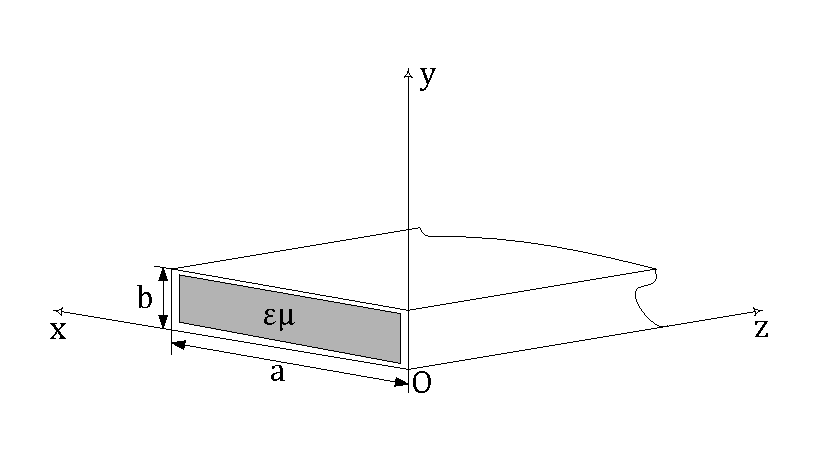
\includegraphics[width=7cm]{Cha6//fig6-3.pdf}
                \caption{矩形波导坐标系}
            \end{figure}
        \end{column}
    \end{columns}
\end{frame}

\begin{frame}{矩形波导}
    \begin{align}
        \frac{\partial^2H_z(x,y)}{\partial x^2}+\frac{\partial^2H_z(x,y)}{\partial y^2}=-k_c^2H_z(x,y)
        \label{eqn6-16}
    \end{align}
    $H_z(x,y)$可分离变量,即$H_z(x,y)=X(x)Y(y)$,(\ref{eqn6-16})可写为
    \begin{align}
        \frac{1}{X}\frac{\rm{d}^2X}{\rm{d}x^2}+\frac{1}{Y}\frac{\rm{d}^2Y}{\rm{d}y^2}=-k_c^2
        \label{eqn6-17}
    \end{align}
    式(\ref{eqn6-17})左边每项都是常数,可得
    \begin{align}
        \begin{cases}
            \dfrac{1}{X}\dfrac{\rm{d}^2X}{\rm{d}x^2}=-k_x^2 \\
            \dfrac{1}{Y}\dfrac{\rm{d}^2Y}{\rm{d}y^2}=-k_y^2 \\
            k_x^2+k_y^2=k_c^2
        \end{cases}
    \end{align}
    一般解为
    \begin{align*}
        X=A\cos(k_x x+\varphi_x);Y=B\cos(k_y y+\varphi_y)
    \end{align*}

\end{frame}

\begin{frame}{矩形波导}
    总的纵向磁场为:
    \begin{align}
        H_z=H_0\cos(k_x x+\varphi_x)\cos(k_y y+\varphi_y)\rm{e}^{-\gamma z}
    \end{align}
    $H_0$在问题中认为是未知数,与具体激励强度有关。
    \begin{align*}
        \begin{cases}
            E_x = -\dfrac{\rm{j}\omega\mu}{k_c^2}\dfrac{\partial H_z}{\partial y}=H_0\dfrac{\rm{j}\omega\mu}{k_c^2}k_y\cos(k_x x+\varphi_x)\sin(k_y y+\varphi_y)\rm{e}^{-\gamma z} \\
            E_y = \dfrac{\rm{j}\omega\mu}{k_c^2}\dfrac{\partial H_z}{\partial x}=-H_0\dfrac{\rm{j}\omega\mu}{k_c^2}k_x\sin(k_x x+\varphi_x)\cos(k_y y+\varphi_y)\rm{e}^{-\gamma z}
        \end{cases}
    \end{align*}
    利用边界条件,即波导4个边壁上电场切向分量为0
    \begin{align*}
        \begin{cases}
            E_y = 0 \qquad x=0,x=a \\
            E_x = 0 \qquad y=0,y=b
        \end{cases}
    \end{align*}
\end{frame}

\begin{frame}{矩形波导}
    \begin{align*}
        \begin{cases}
            x=0,E_y=0 \rightarrow \varphi_x=0                                    \\
            x=a,E_y=0 \rightarrow k_x a=m\pi \rightarrow k_x=\frac{m\pi}{a},m=0,1,2,\cdots \\
            y=0,E_x=0 \rightarrow \varphi_y=0                                    \\
            y=b,E_x=0 \rightarrow k_y b=n\pi \rightarrow k_y=\frac{n\pi}{b},n=0,1,2,\cdots
        \end{cases}
    \end{align*}
    \begin{align}
        \begin{cases}
            H_z=H_0\cos\left(\dfrac{m\pi}{a}x\right)\cos\left(\dfrac{n\pi}{b}y\right)\rm{e}^{-\gamma z}                                             \\
            E_x=\rm{j}\dfrac{\omega\mu}{k_c^2}\dfrac{n\pi}{b}H_0\cos\left(\dfrac{m\pi}{a}x\right)\sin\left(\dfrac{n\pi}{b}y\right)\rm{e}^{-\gamma z}  \\
            E_y=-\rm{j}\dfrac{\omega\mu}{k_c^2}\dfrac{m\pi}{a}H_0\sin\left(\dfrac{m\pi}{a}x\right)\cos\left(\dfrac{n\pi}{b}y\right)\rm{e}^{-\gamma z} \\
            E_z=0                                                                                                           \\
            H_x=\dfrac{\gamma}{k_c^2}\dfrac{m\pi}{a}H_0\sin\left(\dfrac{m\pi}{a}x\right)\cos\left(\dfrac{n\pi}{b}y\right)\rm{e}^{-\gamma z}           \\
            H_y=\dfrac{\gamma}{k_c^2}\dfrac{n\pi}{b}H_0\cos\left(\dfrac{m\pi}{a}x\right)\sin\left(\dfrac{n\pi}{b}y\right)\rm{e}^{-\gamma z}
        \end{cases}
    \end{align}
    
\end{frame}

\begin{frame}{矩形波导}
    \begin{align}
        k_c^2=k_x^2+k_y^2=\left(\frac{m\pi}{a}\right)^2+\left(\frac{n\pi}{b}\right)^2
    \end{align}
    上述$TE$模称为$TE_{mn}$模,其中$m$表示$x$方向变化的半周期数;$n$表示$y$方向变化的半周期数。由于$m=0$及$n=0$时所有场分量才为0,因此
    矩形波导中存在$TE_{m0}$和$TE_{0n}$等波形。若$a>b$,则模$TE_{10}$是最低次波型,其余波型为高次波型。\\
    关于\textbf{本征模}:\\
    以矩形波导为例,尽管在$z$方向它们只可能是入射波加反射波,但是由于横向边界条件的约束,它们由$TE_{mn}$
    和$TM_{mn}$模组成,并且只能由$TE_{mn}$和$TM_{mn}$模组成(后者称为完备性),矩形波导中这些模的完备
    集合就是本征模。
\end{frame}

\begin{frame}{矩形波导}
    同理,对于$TM$模来说$H_z=0$总的纵向电场为:
    \begin{align}
        E_z=E_0\sin\left(\frac{m\pi}{a}x\right)\sin\left(\frac{n\pi}{b}y\right)\rm{e}^{-\gamma z}
    \end{align}
    本征值:
    $$k_x=\frac{m\pi}{a},k_y=\frac{n\pi}{b}\quad m,n=1,2,\cdots$$
    
    \begin{align*}
        \begin{cases}
            E_x = -\rm{j}\dfrac{\beta}{k_c^2}\left(\dfrac{m\pi}{a}\right)E_0\cos\left(\dfrac{m\pi}{a}x\right)\sin\left(\dfrac{n\pi}{b}y\right)\rm{e}^{-\gamma z}\\
            E_y = -\rm{j}\dfrac{\beta}{k_c^2}\left(\dfrac{n\pi}{b}\right)E_0\sin\left(\dfrac{m\pi}{a}x\right)\cos\left(\dfrac{n\pi}{b}y\right)\rm{e}^{-\gamma z}\\
            H_x = \rm{j}\dfrac{\omega\epsilon}{k_c^2}\left(\dfrac{n\pi}{b}\right)E_0\cos\left(\dfrac{m\pi}{a}x\right)\sin\left(\dfrac{n\pi}{b}y\right)\rm{e}^{-\gamma z}\\
            H_y = -\rm{j}\dfrac{\omega\epsilon}{k_c^2}\left(\dfrac{m\pi}{a}\right)E_0\sin\left(\dfrac{m\pi}{a}x\right)\cos\left(\dfrac{n\pi}{b}y\right)\rm{e}^{-\gamma z}\\
            H_z = 0
        \end{cases}
    \end{align*}
\end{frame}

\begin{frame}{矩形波导}
    上述$TM$模称为$TM_{mn}$模,其中$m$表示$x$方向变化的半周期数;$n$表示$y$方向变化的半周期数。由于$m=0$或$n=0$时所有场分量均为0,因此
    矩形波导中不存在$TM_{00}$、$TM_{0n}$及$TM_{m0}$等波形。所以$TM_{11}$是最低次波型,其余波型为高次波型。\\
\end{frame}

\begin{frame}{矩形波导}
    \begin{itemize}
        \item $TE_{10}模$
    \end{itemize}
    即$TE_{mn}$模中下标$m=1,n=0$的情况,是满足$a>b$条件下的矩形波导中\textbf{截止频率}最低的模式,也叫主模。
    \begin{align*}
        \begin{cases}
            H_z=H_0\cos\left(\dfrac{\pi}{a}x\right)\rm{e}^{-\rm{j}\beta z}\\
            E_y=-\rm{j}\dfrac{\omega\mu}{k_c^2}\left(\dfrac{\pi}{a}\right)H_0\sin\left(\dfrac{\pi}{a}x\right)\rm{e}^{-\rm{j}\beta z}\\
            H_x=\dfrac{\rm{j}\beta}{k_c^2}\left(\dfrac{\pi}{a}\right)H_0\sin\left(\dfrac{\pi}{a}x\right)\rm{e}^{-\rm{j}\beta z}
        \end{cases}
    \end{align*}
    只取其实部解,得
    \begin{align*}
        \begin{cases}
            H_z=H_0\cos\left(\dfrac{\pi}{a}x\right)\cos(\omega t-\beta z)\\
            E_y=\dfrac{\omega\mu}{k_c^2}\left(\dfrac{\pi}{a}\right)H_0\sin\left(\dfrac{\pi}{a}x\right)\sin(\omega t-\beta z)\\
            H_x=-\dfrac{\beta}{k_c^2}\left(\dfrac{\pi}{a}\right)H_0\sin\left(\dfrac{\pi}{a}x\right)\sin(\omega t-\beta z)
        \end{cases}
    \end{align*}
\end{frame}

\begin{frame}{矩形波导}
    \begin{itemize}
        \item $TE_{10}$模场结构
    \end{itemize}
    $TE_{10}$模场强与$y$无关,场分量沿$y$轴均匀分布。沿$x$轴的变化规律为:
    $$E_y \propto \sin(\pi x/a),H_x \propto \sin(\pi x/a),H_z \propto \cos(\pi x/a)$$
    \begin{columns}
        \begin{column}{0.7\linewidth}
            \begin{figure}
                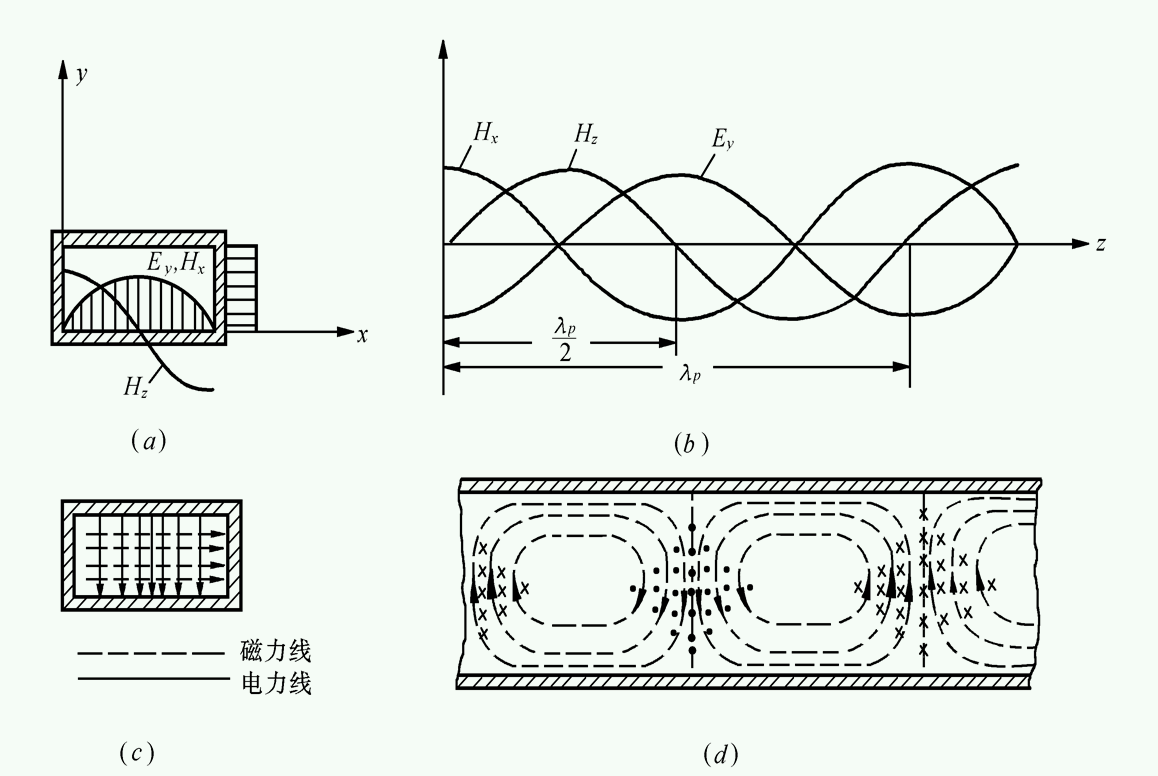
\includegraphics[width=7cm]{Cha6//fig6-4.png}
                \caption{\footnotesize{矩形波导$TE_{10}$模场分量分布规律}}
            \end{figure}
        \end{column}
        \begin{column}{0.3\linewidth}
            {\footnotesize (a)场分量沿$x$轴变化规律\\
            (b)场分量沿$z$轴变化规律\\
            (c)矩形波导横截面场分布\\
            (d)矩形波导纵剖面场分布}
        \end{column}
    \end{columns}
\end{frame}

\begin{frame}{矩形波导}
    某一时刻$TE_{10}$模完整的场分布,随时间推移,场分布图以相速$v_P$沿传输方向移动
    \begin{figure}
        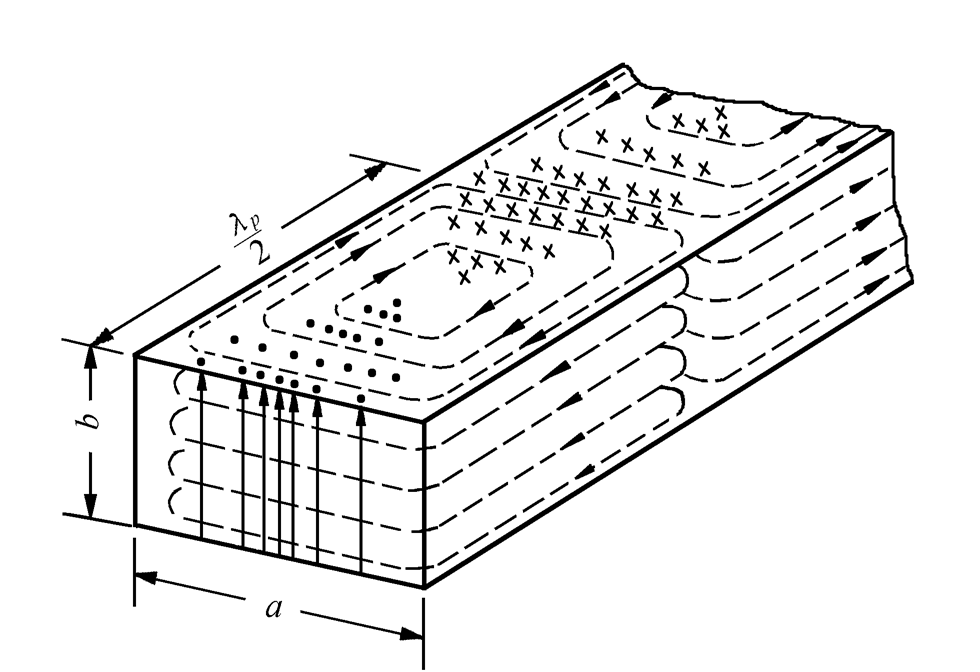
\includegraphics[width=9cm]{Cha6//fig6-5.png}
        \caption{\footnotesize{矩形波导$TE_{10}$模场分布图}}
    \end{figure}
\end{frame}

\begin{frame}{矩形波导}
    \begin{itemize}
        \item 根据导体中电磁波传播,在微波波段,趋肤效应使感应电流在很薄的波导内壁表面流动  ————称为\textbf{壁电流}
    \end{itemize}
    \begin{columns}
        \begin{column}{0.5\linewidth}
            $$\vec{J_S}=\hat{n}\times\vec{H}_{\tan}$$
        \end{column}
        \begin{column}{0.5\linewidth}
            \begin{figure}
                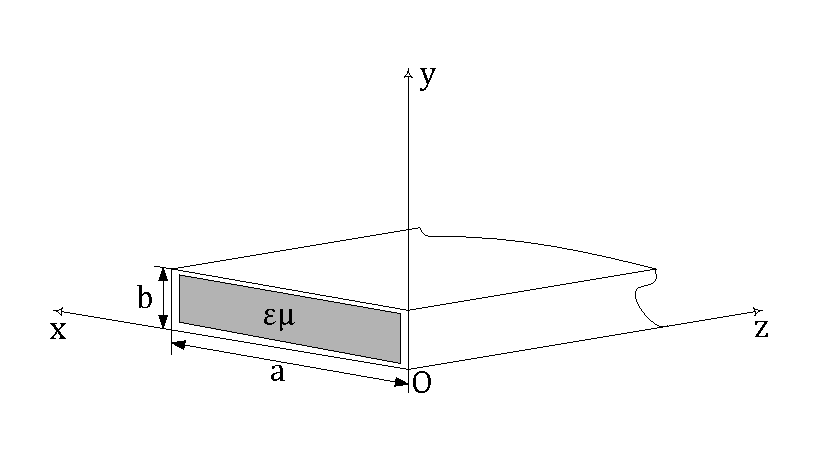
\includegraphics[width=5cm]{Cha6//fig6-3.pdf}
            \end{figure}
        \end{column}
    \end{columns}
    以$TE_{10}$模为例
    \begin{align*}
        \begin{cases}
            \vec{J_S}|_{y=0}=\hat{y}\times[\hat{x}H_x+\hat{z}H_z]_{y=0}=[\hat{x}H_z-\hat{z}H_x]_{y=0}\\
            \vec{J_S}|_{y=b}=-\hat{y}\times[\hat{x}H_x+\hat{z}H_z]_{y=b}=[-\hat{x}H_z+\hat{z}H_x]_{y=b}\\
            \vec{J_S}|_{x=0}=\hat{x}\times\hat{z}H_z|_{x=0}=-\hat{y}H_z|_{x=0}\\
            \vec{J_S}|_{x=a}=-\hat{x}\times\hat{z}H_z|_{x=a}=\hat{y}H_z|_{x=a}
        \end{cases}
    \end{align*}
\end{frame}

\begin{frame}{矩形波导}
    \begin{align*}
        \color{blue}{\vec{J_S}(y=0)=[\hat{x}H_{10}\cos(\pi x/a)-\mathrm{j}\hat{z}\frac{\beta a}{\pi}H_{10}\sin(\pi x/a)]}\\
        \color{blue}{\vec{J_S}(y=b)=[-\hat{x}H_{10}\cos(\pi x/a)+\mathrm{j}\hat{z}\frac{\beta a}{\pi}H_{10}\sin(\pi x/a)]}
    \end{align*}
    \begin{columns}
        \begin{column}{0.5\linewidth}
            \begin{figure}
                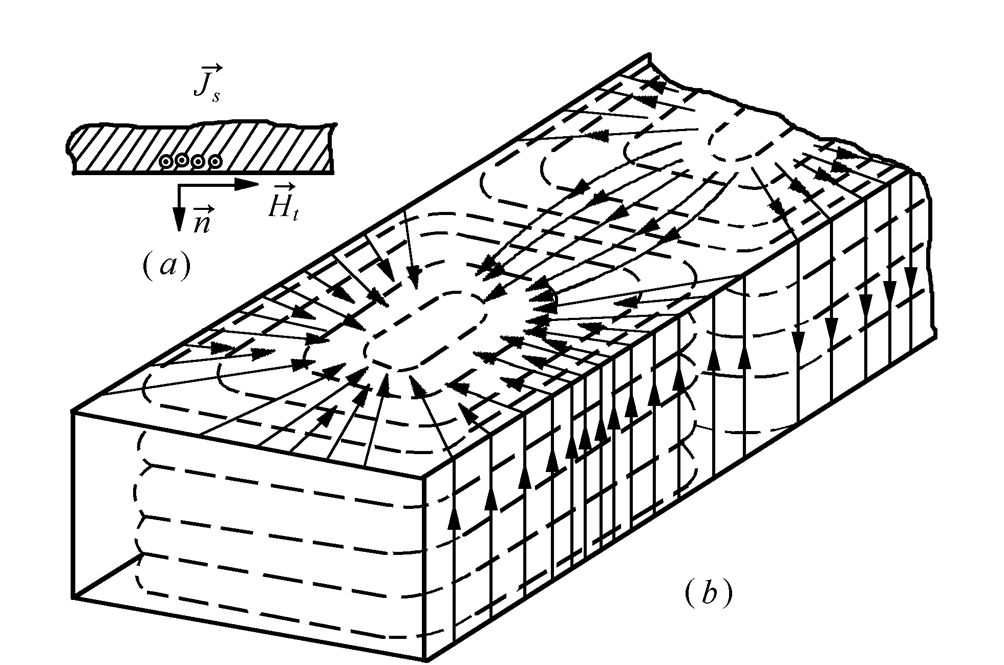
\includegraphics[width=6cm]{Cha6//fig6-6.png}
                \caption{矩形波导$TE_{10}$模管壁电流分布}
            \end{figure}
        \end{column}
        \begin{column}{0.5\linewidth}
            \fbox{面电流与磁力线、表面法向正交}
            \begin{align*}
                \vec{J_S}(x=0)=-\hat{y}H_{10}\\
                \vec{J_S}(x=a)=-\hat{y}H_{10}
            \end{align*}
        \end{column}
    \end{columns}
\end{frame}

\begin{frame}{矩形波导}
    \begin{itemize}
        \item 截止特性
    \end{itemize}
    由于$k_c^2=k^2+\gamma^2=k^2-\beta^2=\left(\frac{m\pi}{a}\right)^2+\left(\frac{n\pi}{b}\right)^2$,
    而传播相位因子$\rm{e}^{-\rm{j}\beta z}$中,如$\beta$需要是实数,必须满足
    $$\beta^2=k^2-k_c^2>0或k>k_c$$
    对于$TE_{10}$模来说,必须要满足
    \begin{align}
        \frac{2\pi}{\lambda}>\frac{\pi}{a}\qquad \lambda<2a
    \end{align}
    为此,定义
    \begin{align}
        k_c=\frac{2\pi}{\lambda_c}
    \end{align}
    其中,$\lambda_c=2a$称为截止波长;$k_c$是对应的截止波数。
\end{frame}

\begin{frame}{矩形波导}
    TE波和TM波的\textbf{截止频率}为
    \begin{align*}
        f_c=\frac{v}{\lambda_c}=\frac{k_c}{2\pi\sqrt{\mu\epsilon}}=\frac{1}{2\sqrt{\mu\epsilon}}\sqrt{\left(\frac{m}{a}\right)^2+\left(\frac{n}{b}\right)^2}
    \end{align*}
    截止波长:
    \begin{empheq}[box=\fbox]{align*}
        \lambda_c=\frac{2\pi}{k_c}=\frac{2}{\sqrt{(m/a)^2+(n/b)^2}}
    \end{empheq}
    截止条件可记为:
    $$f<f_c或\lambda>\lambda_c$$\\
    截止波长不仅与波导尺寸$a$和$b$有关,而且与决定波型的$m$和$n$有关,截止频率还与介质特性有关。在这种意义下,波导是一个\textcolor{blue}{高通}滤波器,“低频”信号无法通过。
\end{frame}

\begin{frame}{矩形波导}
    当波导尺寸$a$和$b$给定时,将不同$m$和$n$值代入,即可得到不同波型的截止波长。其分布如图
    \begin{figure}
        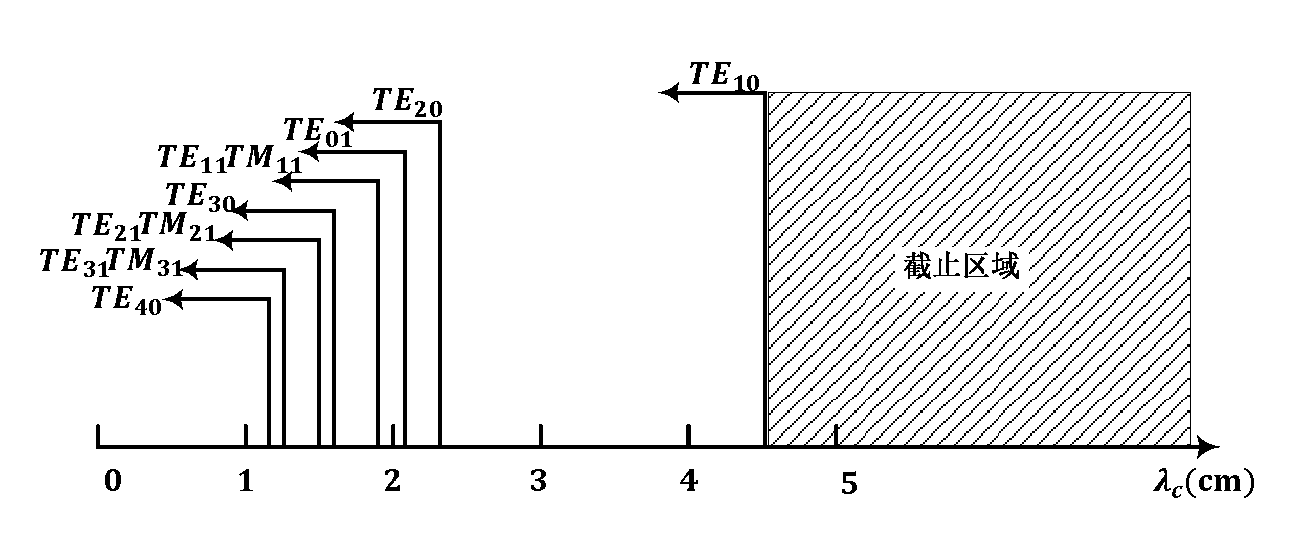
\includegraphics[width=8cm]{Cha6//fig6-7.pdf}
        \caption{BJ-100型波导不同波型截止波长分布图}
    \end{figure}
    从图中可以看到,$TE_{10}$模的截止波长最长,右边的阴影区为截止区。
\end{frame}

\begin{frame}{矩形波导}
    \begin{itemize}
        \item 模式简并
    \end{itemize}
    不同导模的截止波长$\lambda_c$相同现象\\
    相同的波型指数$m$和$n$的$TE_{mn}$和$TM_{mn}$的截止波长相同,矩形波导的导模具有双重简并。
    \begin{itemize}
        \item 主模$TE_{10}$模——主模
        \begin{enumerate}
            \item 通常矩形波导工作在$TE_{10}$单模传输情况,因为$TE_{10}$模容易实现单模传输。
            \item 当工作频率一定时传输$TE_{10}$模的波导尺寸最小
            \item 若波导尺寸一定,则实现单模传输的频带最宽。
        \end{enumerate}
    \end{itemize}
    为了实现$TE_{10}$单模传输,则要求电磁波的工作波长必须满足下列条件
    \begin{align*}
        \begin{cases}
            \lambda_c(TE_{20})<\lambda<\lambda_c(TE_{10})\\
            \lambda>\lambda_c(TE_{01})
        \end{cases}
        \rightarrow
        \begin{cases}
            a<\lambda<2a\\
            \lambda>2b
        \end{cases}
    \end{align*}
    当工作波长给定时,若要实现$TE_{10}$单模传输,则波导尺寸必须满足
    $$\lambda/2<a<\lambda \quad b<\lambda/2$$
\end{frame}

\begin{frame}{矩形波导}
    \begin{itemize}
        \item 波导波长$\lambda_g$
    \end{itemize}
    \begin{align}
        \lambda_g=\frac{\lambda}{\sqrt{1-\left(\frac{\lambda}{\lambda_c}\right)^2}}
    \end{align}
    很明显,波导波长$\lambda_g$大于自由空间波长$\lambda$。设传播常数$\beta=\dfrac{2\pi}{\lambda_g}$,则有
    $$\beta^2=k^2-k_c^2=\left(\frac{2\pi}{\lambda}\right)^2-\left(\frac{2\pi}{\lambda_c}\right)^2=\left(\frac{2\pi}{\lambda_g}\right)^2$$
    即可推导得
    $$\lambda_g=\frac{\lambda}{\sqrt{1-\left(\frac{\lambda}{\lambda_c}\right)^2}}=\frac{\lambda}{\sqrt{1-\left(\frac{\lambda}{2a}\right)^2}}$$
\end{frame}

\begin{frame}{矩形波导}
    \begin{itemize}
        \item 相速$v_p$
    \end{itemize}
    \begin{align}
        v_p=\frac{c}{\sqrt{1-\left(\frac{\lambda}{\lambda_c}\right)^2}}=\frac{c}{\sqrt{1-\left(\frac{\lambda}{2a}\right)^2}}>c
    \end{align}
    已知相位因子构成的等相位面
    \begin{align*}
        \omega t-\beta z=const \\
        v_p=\frac{\rm{d}z}{\rm{d}t}=\frac{\omega}{\beta}=\frac{2\pi c/\lambda}{2\pi/\lambda_g}=c\frac{\lambda_g}{\lambda} \\
           =\frac{c}{\sqrt{1-\left(\frac{\lambda}{\lambda_c}\right)^2}}=\frac{c}{\sqrt{1-\left(\frac{\lambda}{2a}\right)^2}} 
    \end{align*}
    显然相速$v_p$大于自由空间光速,但相速并不是能量传播速度。
\end{frame}

\begin{frame}{矩形波导}
    \begin{itemize}
        \item 群速$v_g$
    \end{itemize}
    \begin{align*}
        v_g&=\frac{\rm{d}\omega}{\rm{d}\beta}\\
        \beta &= \sqrt{k^2-k_c^2}=\sqrt{\omega^2\epsilon\mu-k_c^2}\\
        \frac{\rm{d}\beta}{\rm{d}\omega}&=\frac{1}{2}\frac{2\omega\epsilon\mu}{\sqrt{k^2-k_c^2}}=\frac{k^2/\omega}{\sqrt{k^2-k_c^2}}=\frac{v_p}{c^2}
    \end{align*}
    \begin{align}
        v_g = \frac{c^2}{v_p}=c\sqrt{1-\left(\frac{\lambda}{\lambda_c}\right)^2}=c\sqrt{1-\left(\frac{\lambda}{2a}\right)^2}<c
    \end{align}
    \begin{align}
        v_p v_g=c^2
    \end{align}
\end{frame}

\begin{frame}{矩形波导}
    \begin{itemize}
        \item 波型阻抗
    \end{itemize}
    \begin{align}
        \eta_{TE}=\left|\frac{E_t}{H_t}\right|=\frac{\omega\mu}{\beta}=\sqrt{\frac{\mu}{\epsilon}}\frac{k}{\beta}=\eta\frac{\lambda_g}{\lambda}=\eta\frac{1}{\sqrt{1-\left(\frac{\lambda}{\lambda_c}\right)^2}}\\
        \color{blue}{\eta_{TE_{10}}=\left|\frac{E_y}{H_x}\right|=\sqrt{\frac{\mu}{\epsilon}}\bullet\frac{1}{\sqrt{1-\left(\frac{\lambda}{2a}\right)^2}}}\\
        \eta_{TM}=\left|\frac{E_t}{H_t}\right|=\frac{\beta}{\omega\epsilon}=\sqrt{\frac{\mu}{\epsilon}}\frac{\beta}{k}=\eta\sqrt{1-\left(\frac{\lambda}{\lambda_c}\right)^2}
    \end{align}
\end{frame}

\subsection{圆波导}
\begin{frame}{圆波导}

\end{frame}

\subsection{同轴线}
\begin{frame}{同轴线}

\end{frame}

\subsection{平面传输线}
\begin{frame}{平面传输线}
    上世纪六十年代以来,在微波工程和微波技术上,出现了一次不小的革命,即所谓MIC(Microwave Integrated Circuit)微波集成电路——HMIC、MMIC。其特色是体积小、功能多、频带宽,但承受功率小。因此被广泛应用于接收机和小功率元件中,并都传输TEM波。\\
    作为这一革命的“过渡人物”是带状线(Stripline)。它可以看作是同轴线的变形。
\end{frame}






